%!TEX root = main.tex
\section{Warm-up:  2-Level Explore-then-Exploit Policy}
\swedit{Now we provide a simple policy that can incentivize the agents
  to perform non-adaptive exploration and achieve a regret rate of
  $\tilde O(T^{2/3})$. The policy essentially follows the
  ``explore-then-exploit'' paradigm and consists two phases, which can
  be described as a two-level information graph (as shown in
  Figure~\ref{fig:2level}).  In the first level, we perform
  exploration by simulating $T_1$ independent runs \ALGG of $\GdT$
  rounds. This is done by randomly dividing the first $T_1 \cdot \GdT$
  agents into $T_1$ groups of equal size and each agent only observe
  the history of all previous agents in the same group.  In the second
  level, we ``exploit'' by showing all the remaining agents the entire
  history of first phase.

  The key idea behind the policy is that the first level effectively
  boosts the exploration probability of Greedy. Since each run of
  \ALGG explores all arms with constant probability (Lemma
  \ref{lem:greedy}), by simulating multiple runs of Greedy, we can
  ensure that with high probability, every arm is pulled with a
  sufficient number of times. As a result, every agent in the second
  level will pull an arm with mean rewards close to the optimal.

}





\iffalse
The 2-level recommendation policy is constructed as following.
In the first level, we run $T_1$ \ALGG of $\GdT$ rounds ``in parallel''. More specifically, we divide the first $T_1 \cdot \GdT$ agents into $T_1$ groups of equal size and agents only observe the history of all previous agents in the same group.
In the second level, we show the rest $T-T_1\cdot \GdT$ agents the history of first $T_1 \cdot \GdT$ rounds. We will pick $T_1$ in Theorem \ref{thm:2level}. 
See also Figure \ref{fig:2level} for a graphical view of the information flow.

The idea of this 2-level recommendation policy is simple. We first try to explore all arms enough amount of times in the first level using multiple runs of \ALGG under the guarantee of Lemma \ref{lem:greedy}. After that, by concentration argument, we can show that while observing the history of the first level, agents in the second level pick an arm with mean close to the best arm's mean. 
\fi





\begin{figure}[H]
\centering
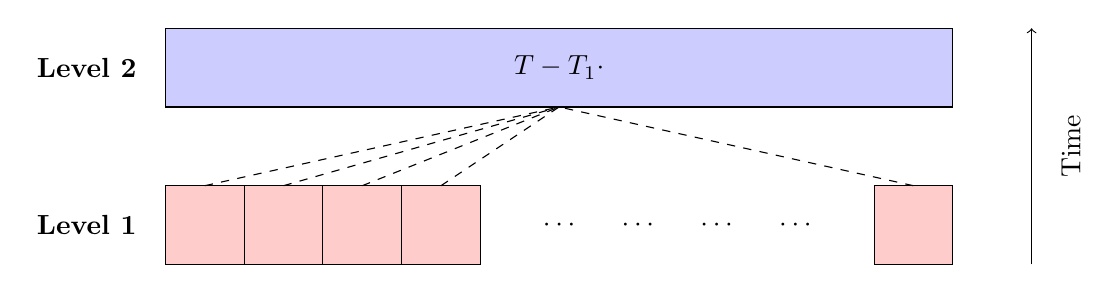
\begin{tikzpicture}  
 \filldraw[fill=blue!20!white]
 (0,2)--(10,2)--(10,3)--(0,3)--cycle;
  \filldraw[fill=red!20!white]
  (0,0)--(1,0)--(1,1)--(0,1)--cycle;
  \draw[dashed] (0.5,1)--(5,2);
  \filldraw[fill=red!20!white]
  (1,0)--(2,0)--(2,1)--(1,1)--cycle;
  \draw[dashed] (1.5,1)--(5,2);
  \filldraw[fill=red!20!white]
  (2,0)--(3,0)--(3,1)--(2,1)--cycle;
  \draw[dashed] (2.5,1)--(5,2);
  \filldraw[fill=red!20!white]
  (3,0)--(4,0)--(4,1)--(3,1)--cycle;
  \draw[dashed] (3.5,1)--(5,2);
  \filldraw[fill=red!20!white]
  (9,0)--(10,0)--(10,1)--(9,1)--cycle;
  \draw[dashed] (9.5,1)--(5,2);
  \node at(5,0.5){$\cdots$};
  \node at(6,0.5){$\cdots$};
  \node at(7,0.5){$\cdots$};
  \node at(8,0.5){$\cdots$};
  \node at(5,2.5){$T -T_1 \cdot \GdT$};
  \node at(0.5,0.5){$\GdT$};
  \node at(1.5,0.5){$\GdT$};
  \node at(2.5,0.5){$\GdT$};
  \node at(3.5,0.5){$\GdT$};
  \node at(9.5,0.5){$\GdT$};
  \node at(-1,0.5){\textbf{Level 1}};
  \node at(-1,2.5){\textbf{Level 2}};
  \draw[->] (11,0)--(11,3);
  \node at(11.5,1.5)[ rotate=90]{Time};
\end{tikzpicture}

\caption{Structure of information graph for the 2-level policy. Each
  red ``box'' is level 1 corresponds to a path connecting a set of
  $T_G$ agents. The entire history in level 1 is then aggregated and
  shown to each agent in level 2.}
\label{fig:2level}
\end{figure}

\begin{theorem}
\label{thm:2level}
With proper setting of $T_1$, the 2-level policy gets expected regret
$O(T^{2/3} \log(T)^{1/3})$. If we know the gap between the means of
the best arm and second best arm is larger than $\Delta$, we can make
the expected regret $O(\log(T) \cdot \Delta^{-2})$.
\end{theorem}

\swcomment{I think this proof should go to appendix, so I didn't do
  too much refactoring}

\begin{proof}
  We will set $T_1$ later in the proof, depending on whether the gap
  parameter $\Delta$ is known. For now, we just need to know we will
  make $T_1 \geq \frac{4\GdT^2}{\GdP^2}\log(T)$. Since this policy is
  agnostic to the indices of the arms, we assume w.l.o.g. that arm 1
  has the highest mean.

  The first $T_1 \cdot \GdT$ rounds will get total regret at most
  $T_1 \cdot \GdT$.  We focus on bounding the regret from the second
  level of $T - T_1 \cdot \GdT$ rounds. We consider the following two
  clean events. We will first bound the probability that both of them
  happen and then we will show that they together imply upper bounds
  on $|\hat{\mu}^t_a - \mu_a|$'s for any agent $t$ in the second
  level. Recall $\hat{\mu}^t_a$ is the estimated mean of arm $a$ by
  agent $t$ and agent $t$ picks the arm with the highest
  $\hat{\mu}^t_a$.

% \begin{itemize}
  \paragraph{Concentration of the number of arm $a$ pulls in the first
    level.}
  For each arm $a$, define $q_a$ to be the expected number of arm $a$
  pulls in a single run of \ALGG used in the first level.  By Lemma
  \ref{lem:greedy}, we know $\GdP \leq q_a \leq \GdT$. Define $W_1^a$
  to be the event that the number of arm $a$ pulls in the first level
  is at least $q_a T_1- \GdT \sqrt{T_1\log(T)}$.  \swedit{As long as
    we set $T_1 \geq \frac{4\GdT^2}{\GdP^2}\log(T)$, this implies that
    the number of arm $a$ pulls is then at least $q_a T_1/2$.}  By
  Chernoff bound,
  \[
    \Pr[W_1^a] \geq 1-\exp(-2\log(T)) \geq 1-1/T^2.
  \]
Define $W_1$ to be the intersection of all these events (i.e. $W_1 = \bigcap_{a}W_1^a$). By union bound, we have
\[
\Pr[W_1] \geq 1- \frac{K}{T^2} \geq 1 - \frac{1}{T}.
\]
\paragraph{Concentration of the empirical mean of arm $a$ pulls in the first level.}
To facilitate our reasoning, let us imagine there is a tape of length
$T$ for each arm $a$, with each cell containing an independent draw of
the realized reward from the distribution Ber$(\mu_a)$. Then for each
arm $a$ and any $N\in [T]$, we can think of the sequence of the first
$N$ realized rewards of $a$ coming from the prefix of $N$ cells in its
reward tape. Define $W^{a,t}_2$ to be the event that the empirical
mean of the first $t$ \swedit{realized rewards in the tape} of arm $a$
is at most $\sqrt{\frac{2\log(T)}{t}}$ away from $\mu_a$. Define $W_2$
to be the intersection of these events (i.e.
$\bigcap_{a,t} W^{a,t}_2$).  By Chernoff bound,\swcomment{$t$ may be
  confusing here}
\[
\Pr[W^{a,t}_2] \geq 1 - 2\exp(-4\log(T)) \geq 1-2/T^4.
\]
By union bound, 
\[
\Pr[W_2] \geq 1 - KT \cdot \frac{2}{T^4} \geq 1 - \frac{2}{T}.
\]



By union bound, we know $\Pr[W_1 \cap W_2] \geq 1 - 3/T$. For the
remainder of the analysis, we will condition on the event
$W_1 \cap W_2$.

For any arm $a$ and agent $t$ in the second level, by $W_1$ and $W_2$, we have
\[
|\bar{\mu}^t_a - \mu_a| \leq \sqrt{\frac{2\log(T)}{q_aT_1 /2}}.
\]
By $W_1$ and Assumption \ref{ass:embehave}, we have
\[
|\bar{\mu}^t_a - \hat{\mu}^t_a| \leq \frac{c_m}{\sqrt{q_aT_1/2}}.
\]
Therefore,
\[
|\hat{\mu}^t_a - \mu_a|\leq \sqrt{\frac{2\log(T)}{q_aT_1 /2}}+\frac{c_m}{\sqrt{q_aT_1/2}} \leq 3 \sqrt{\frac{\log(T)}{\GdP T_1 }}.
\]
So the second-level agents will pick an arm $a$ which has $\mu_a$ at most $6 \sqrt{\frac{\log(T)}{\GdP T_1 }}$ away from $\mu_1$. To sum up, the total expected regret is at most 
\[
T_1 \cdot \GdT + T \cdot (1-\Pr[W_1 \cap W_2]) + T \cdot  6 \sqrt{\frac{\log(T)}{\GdP T_1 }}.
\]
By setting $T_1 = T^{2/3}\log(T)^{1/3}$, we get expected regret $O(T^{2/3}\log(T)^{1/3})$.

Notice that if we know the gap parameter is known to be larger than
$\Delta$, we can set
\[
T_1 = \max\left( \frac{4\GdT^2}{\GdP^2}\log(T), \frac{36 }{\Delta^2 \cdot p_G} \log(T) \right).
\]
In this case, since $\Delta \geq 6 \sqrt{\frac{\log(T)}{\GdP T_1 }}$, we know agents in the second level will all pull arm 1. Therefore, the total expected regret is at most
\[
T_1 \cdot \GdT + T \cdot (1- \Pr[W_1 \cap W_2]) = O(\Delta^{-2} \log(T)).
\]
This completes the proof.
\end{proof}
%%% Local Variables:
%%% mode: latex
%%% TeX-master: "main"
%%% End:
